\section{Project Discovery}\label{sec:project_discovery}
In this section we discuss the status of the game as it was at the beginning of the project, and outline the game itself.\\

\subsection{The beginning}
When the project began, the newest user interface design had been decided, and the game had around half of that design already implemented. As is seen on figure \ref{fig:PD}.

\begin{figure}[H]
	\centering
	\graphicspath{ {./graphics/} }
    \centerline{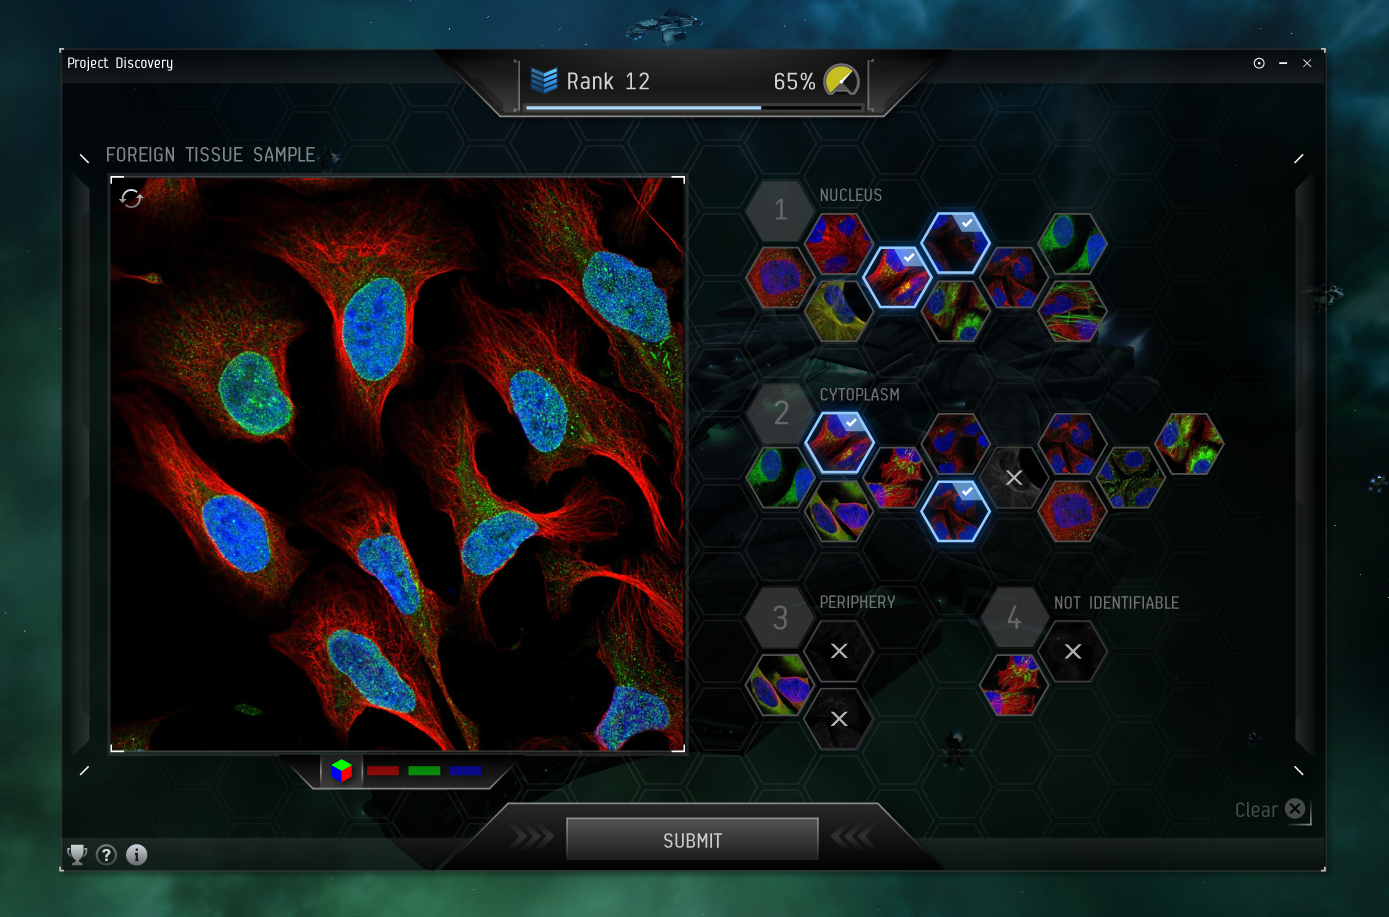
\includegraphics[scale=0.35]{PD.png}}
    \caption{\label{fig:PD}The design of the UI as the project began}
\end{figure}
\clearpage

The game also already had a few features implemented, such as players being able to receive images, selecting their appropriate categories and submitting their classifications. A simple rewarding system was also already in place, rewarding players with in game currency (ISK), experience points (XP) and loyalty points (LP) when players submitted a solution. They then got a reward based on their score for the image they just classified, but since those images were 'training images', we knew the solution and could grade the player on that. However, that needed to be changed later on because when the client got an image that we did not know the solution for, no reward was given. Finally, a rudamentary tutorial phase was implemented, but it was too small and needed to be expanded to improve new player experience.\\

\subsection{The goal}
Stuff...

